\documentclass{memoir}

\usepackage[top=1in,bottom=1in,left=1in,right=1in,letterpaper]{geometry}
\usepackage{graphicx}

\begin{document}
\frontmatter
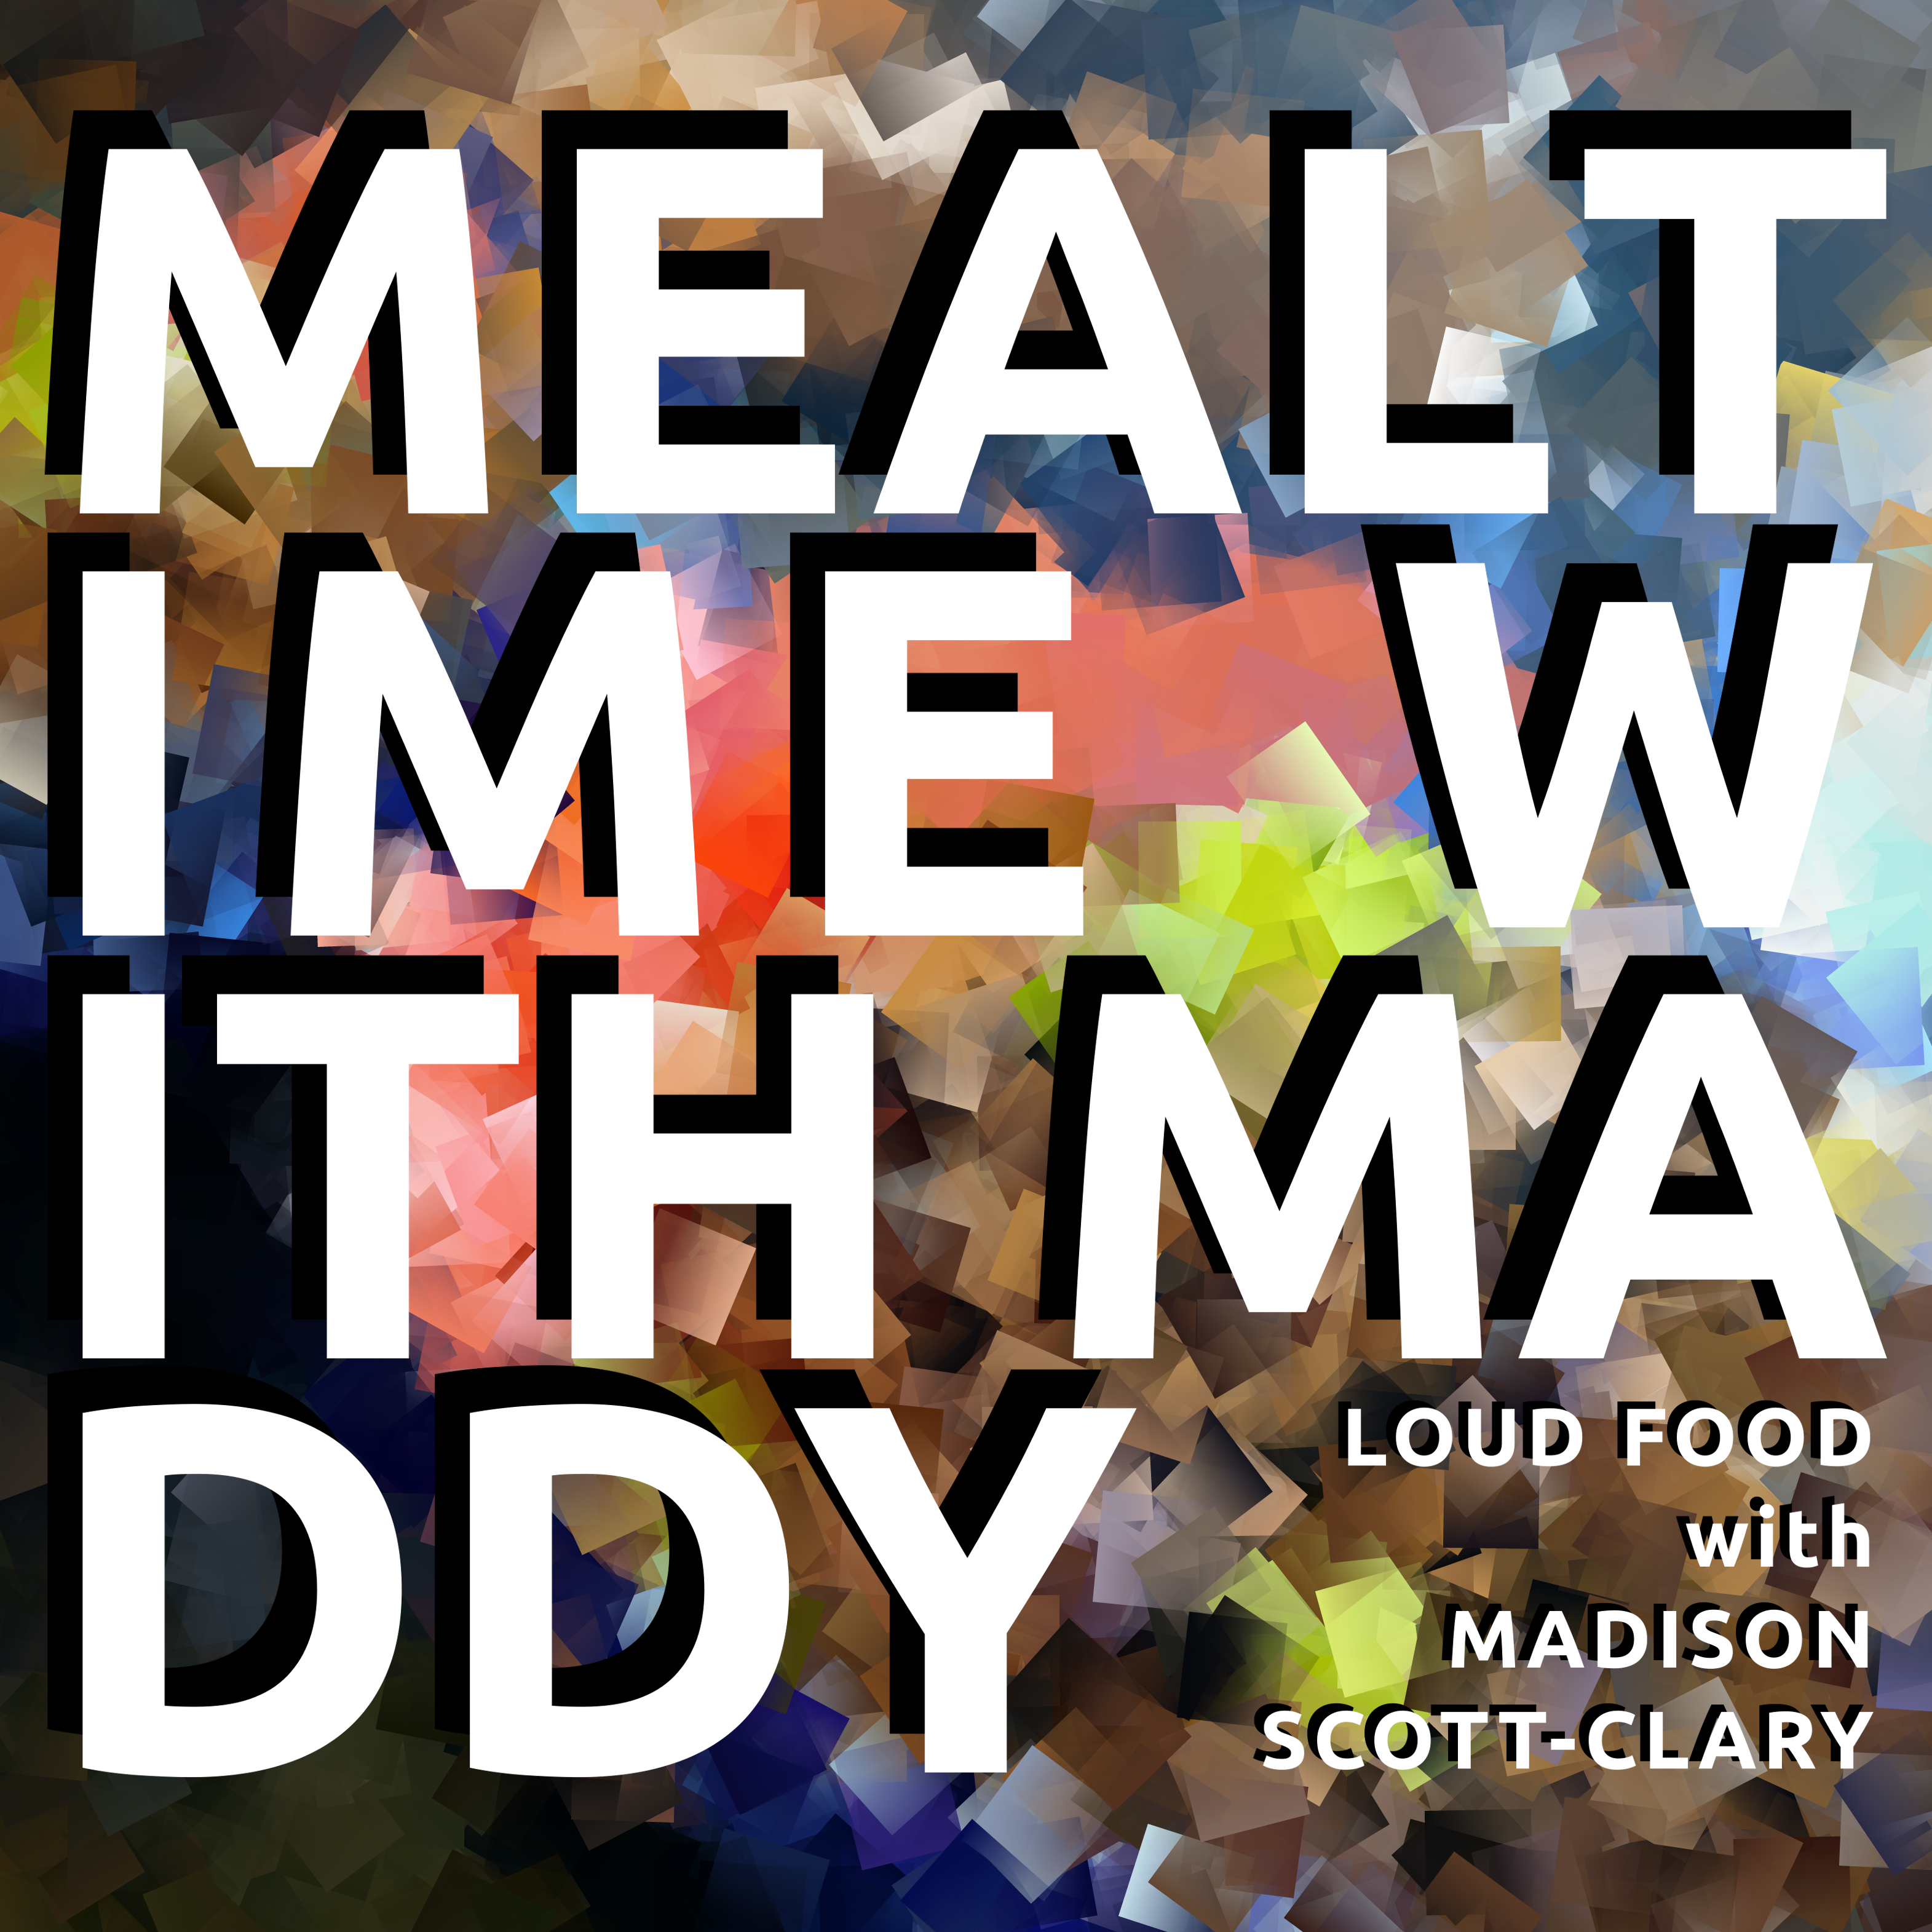
\includegraphics[width=\textwidth]{cover.png}
\thispagestyle{empty}
\newpage

\includegraphics[width=\textwidth]{inner-cover.png}
\thispagestyle{empty}
\newpage

% Title page

\tableofcontents*

\chapter*{Dedication}

\begin{verse}
  To the polycule\\
  \vin JD and Robin and Lexy\\
  To Jenn\\
  To the dogs\\
  \vin Zephyr and Falcon\\
  and to the idea\\
  \vin if not exactly the implementation\\
  \vin \vin of Twitter.
\end{verse}

\chapter{About}

\mainmatter

\chapter*{Ghee}
\renewcommand{\chaptertitle}{Ghee}
\addcontentsline{toc}{chapter}{\hspace{1.5ex}Ghee}


\chapter{Dal}


\chapter{Preserved Lemons --- Part 1}


\chapter{Summer Salad}


\chapter{Tabbouleh}

TIP fried


\chapter*{Preserved Lemons: Part 2}
\renewcommand{\chaptertitle}{Preserved Lemons: Part 2}
\addcontentsline{toc}{chapter}{\hspace{1.5ex}Preserved Lemons: Part 2}


\chapter*{Shakshouka}
\renewcommand{\chaptertitle}{Shakshouka}
\addcontentsline{toc}{chapter}{\hspace{1.5ex}Shakshouka}


\chapter*{Tamago Kake Gohan}
\renewcommand{\chaptertitle}{Tamago Kake Gohan}
\addcontentsline{toc}{chapter}{\hspace{1.5ex}Tamago Kake Gohan}

TIP reheating rice


\chapter{Kimchi --- Part 1}

Getting baek kimchi to spice/age, getting mulkimchi to salt and wait


\chapter*{Juk}
\renewcommand{\chaptertitle}{Juk}
\addcontentsline{toc}{chapter}{\hspace{1.5ex}Juk}


\chapter*{Kimchi: Part 2}
\renewcommand{\chaptertitle}{Kimchi: Part 2}
\addcontentsline{toc}{chapter}{\hspace{1.5ex}Kimchi: Part 2}

Finishing mulkimchi prep with broth, flip baek kimchi


\chapter{Sichuan Dry-Fried String Beans}

TIP make extra oil


TIP make extra oil

\chapter{Kimchi --- Part 3}

jarring baek kimchi


Jarring baek kimchi

\chapter*{Mul-Naengmyeon}
\renewcommand{\chaptertitle}{Mul-Naengmyeon}
\addcontentsline{toc}{chapter}{\hspace{1.5ex}Mul-Naengmyeon}

Using mulkimchi

\newpage
Testing a new page!

\newpage

Wow


Using mulkimchi

\chapter{Okonomiyaki}

TIP using kimchi for kimchijeon


TIP use baek kimchi

\chapter{Orange Sauce}


\chapter*{Green Chili}
\renewcommand{\chaptertitle}{Green Chili}
\addcontentsline{toc}{chapter}{\hspace{1.5ex}Green Chili}

TIP snazzy beans


\chapter{Snazzy Beans}


\chapter*{Preserved Lemons: Part 3}
\renewcommand{\chaptertitle}{Preserved Lemons: Part 3}
\addcontentsline{toc}{chapter}{\hspace{1.5ex}Preserved Lemons: Part 3}


\chapter{Mac \& Cheese}


\chapter*{Bananas Foster}
\renewcommand{\chaptertitle}{Bananas Foster}
\addcontentsline{toc}{chapter}{\hspace{1.5ex}Bananas Foster}


\end{document}
